\hypertarget{patterns-of-peeragogy}{%
\subsection{Patterns of Peeragogy}\label{patterns-of-peeragogy}}

This chapter outlines an approach to the organization of learning that
draws on the principles of free/libre/open source software (FLOSS), free
culture, and peer production. Mako Hill suggests that one recipe for
success in peer production is to take a familiar idea -- for example, an
encyclopedia -- and make it easy for people to participate in building
it {{[}11{]}}. We will take hold of ``learning in institutions'' as a
map, although it does not fully conform to our chosen tacitly-familiar
territory of \emph{peeragogy}. To be clear, peeragogy is for \emph{any
group of people who want to learn anything}.\footnote{\url{https://www.youtube.com/watch?v=TDRGJzoNbAc}}

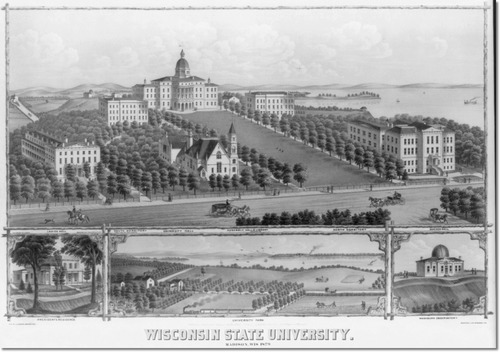
\includegraphics{images/wisconsin-map.jpg}\\
\emph{A prototypical university. Caption reads: Wisconsin State
University, Madison, Wis. 1879. Inset captions describe the pictured
buildings: Ladies Hall, South Dormitory, University Hall, Assembly Halls
\& Library, North Dormitory, Science Hall, President's Residence,
University Farm, and Washburn Observatory. Public domain.}

Despite thinking about learning and adaptation that may take place far
outside of formal institutions, the historical conception of a
university helps give shape to our inqury. The model university is not
separate from the life of the state or its citizenry, but aims to
``assume leadership in the application of knowledge for the direct
improvement of the life of the people in every sphere'' {{[}8{]}}.
Research that \emph{adds to the store of knowledge} is another
fundamental obligation of the university {{[}8{]}}. The university
provides a familiar model for collaborative knowledge work but it is not
the only model available. Considering the role of collaboration in
building Wikipedia, StackExchange, and free/libre/open source software
development, we may be led to ask: What might an accredited
free/libre/open university look like? How would it compare or contrast
with the typical or stereotypical image of a university from the figure
above? Would it have similar structural features, like a Library,
Dormitory, Science Hall and so on? Would participants take on familiar
roles {{[}5{]}}? How would it compare with historical efforts like the
Tuskegee Institute that involved students directly in the production of
physical infrastructure {{[}7,19{]}}? We use the word \emph{peeragogy}
to talk about collaboration in relatively non-hierarchical settings.
Examples are found in education, but also in business, government,
volunteer, and NGO settings. Peeragogy involves both problem solving and
problem definition. Indeed, in many cases it is preferable to focus on
solutions, since people know the ``problems'' all too well {{[}2{]}}.
Participants in a peeragogical endeavor collaboratively build emergent
structures that are responsive to their changing context, and that in
turn, change that context. In the Peeragogy project, we are developing
the the theory and practice of peeragogy.

\emph{Design patterns} offer a methodological framework that we have
used to clarify our focus and organize our work. A design pattern
expresses a commonly-occurring problem, a solution to that problem, and
rationale for choosing this solution {{[}13{]}}. This skeleton is
typically fleshed out with a \emph{pattern template} that includes
additional supporting material; individual patterns are connected with
each other in a \emph{pattern language}. What we present here is rather
different from previous pattern languages that touch on similar topics
-- like \emph{Liberating Voices} {{[}17{]}}, \emph{Pedagogical Patterns}
{{[}3{]}}, and \emph{Learning Patterns} {{[}12{]}}. At the level of the
pattern template, our innovation is simply to add a ``What's next''
annotation, which anticipates the way the pattern will continue to
``resolve''.

This addition mirrors the central considerations of our approach, which
is all about human interaction, and the challenges, fluidity and
unpredictability that come with it. Something that works for one person
may not work for another or may not even work for the same person in a
slightly different situation. We need to be ready to clarify and adjust
what we do as we go. Even so, it is hard to argue with a
sensible-sounding formula like ``If W applies, do X to get Y.'' In our
view, other pattern languages often achieve this sort of common sense
rationality, and then stop. Failure in the prescriptive model only
begins when people try to define things more carefully and make
context-specific changes -- when they actually try to put ideas into
practice. The problem lies in the inevitable distance between \emph{do
as I say}, \emph{do as I do}, and \emph{do with me} {{[}9{]}}. If people
are involved, things get messy. They may think that they are on the same
page, only to find out that their understandings are wildly different.
For example, everyone may agree that the group needs to go ``that way.''
But how far? How fast? It is rare for a project to be able to set or
even define all of the parameters accurately and concisely at the
beginning. And yet design becomes a ``living language'' {{[}1{]}} just
insofar as it is linked to action. Many things have changed since
Alexander suggested that ``you will get the most `power' over the
language, and make it your own most effectively, if you write the
changes in, at the appropriate places in the book'' {{[}1{]}}. We see
more clearly what it means to inscribe the changing form of design not
just in the margins of a book, or even a shared wiki, but in the
lifeworld itself. Other recent authors on patterns share similar views
{{[}15,16,18{]}}.

Learning and collaboration are of interest to both organizational
studies and computer science, where researchers are increasingly making
use of social approaches to software design and development, as well as
agent-based models of computation {{[}6,14{]}}. The design pattern
community in particular is very familiar with practices that we think of
as peeragogical, including shepherding, writers workshops, and design
patterns themselves {{[}4,10,13{]}}.

\hypertarget{pattern-template}{%
\subsection{Pattern template}\label{pattern-template}}

The table below shows the pattern template that we use to present our
patterns. Along with the traditional design patterns components
{{[}13{]}}, each of our patterns is fleshed out with two illustrative
examples. The first is descriptive, and looks at how the pattern applies
in current Wikimedia projects. We selected Wikimedia as a source of
examples because the project is familiar, a demonstrated success, and
readily accessible. The second example shows how the pattern could be
applied in the design of a future university. Each pattern concludes
with a boxed annotation: ``\emph{What's Next in the Peeragogy
Project}''.

\begin{longtable}[]{@{}l@{}}
\toprule
\begin{minipage}[b]{0.97\columnwidth}\raggedright
Pattern template\strut
\end{minipage}\tabularnewline
\midrule
\endhead
\begin{minipage}[t]{0.97\columnwidth}\raggedright
\emph{Motivation} for using this pattern.\strut
\end{minipage}\tabularnewline
\begin{minipage}[t]{0.97\columnwidth}\raggedright
\emph{Context} of application.\strut
\end{minipage}\tabularnewline
\begin{minipage}[t]{0.97\columnwidth}\raggedright
\emph{Forces} that operate within the context of application, each with
a mnemonic glyph.\strut
\end{minipage}\tabularnewline
\begin{minipage}[t]{0.97\columnwidth}\raggedright
\emph{Problem} the pattern addresses.\strut
\end{minipage}\tabularnewline
\begin{minipage}[t]{0.97\columnwidth}\raggedright
\emph{Solution} to the problem.\strut
\end{minipage}\tabularnewline
\begin{minipage}[t]{0.97\columnwidth}\raggedright
\emph{Rationale} for this solution.\strut
\end{minipage}\tabularnewline
\begin{minipage}[t]{0.97\columnwidth}\raggedright
\emph{Resolution} of the forces, named in bold.\strut
\end{minipage}\tabularnewline
\begin{minipage}[t]{0.97\columnwidth}\raggedright
\emph{Example 1}: How the pattern manifests in current Wikimedia
projects.\strut
\end{minipage}\tabularnewline
\begin{minipage}[t]{0.97\columnwidth}\raggedright
\emph{Example 2}: How the pattern could inform the design of a future
university.\strut
\end{minipage}\tabularnewline
\begin{minipage}[t]{0.97\columnwidth}\raggedright
\emph{What's Next in the Peeragogy Project}: How the pattern relates to
our collective intention in the Peeragogy project\strut
\end{minipage}\tabularnewline
\bottomrule
\end{longtable}

\hypertarget{a-short-motivating-example}{%
\subsection{A short motivating
example}\label{a-short-motivating-example}}

When one relative {{Newcomer}} was still in the onboarding process in
Peeragogy project, she hit a wall in understanding the ``patterns''
section in the \emph{Peeragogy Handbook} v1. A more seasoned peer
invited her to a series of separate discussions with their own
{{Heartbeat}} to flesh out the patterns and make them more accessible.
At that time the list of patterns was simply a list of paragraphs
describing recurrent trends. During those sessions, the impact and
meaning of patterns captured her imagination. She went on to become the
champion for the pattern language and its application in the Peeragogy
project. During a ``hive editing'' session, she proposed the template we
initially used to give structure to the patterns. She helped further
revise the pattern language for the \emph{Peeragogy Handbook} v3, and
attended PLoP 2015. While a new domain can easily be overwhelming, this
newcomer found {{A specific project}} to start with, and scaffolded her
knowledge and contributions from that foundation.

\begin{figure}
\centering
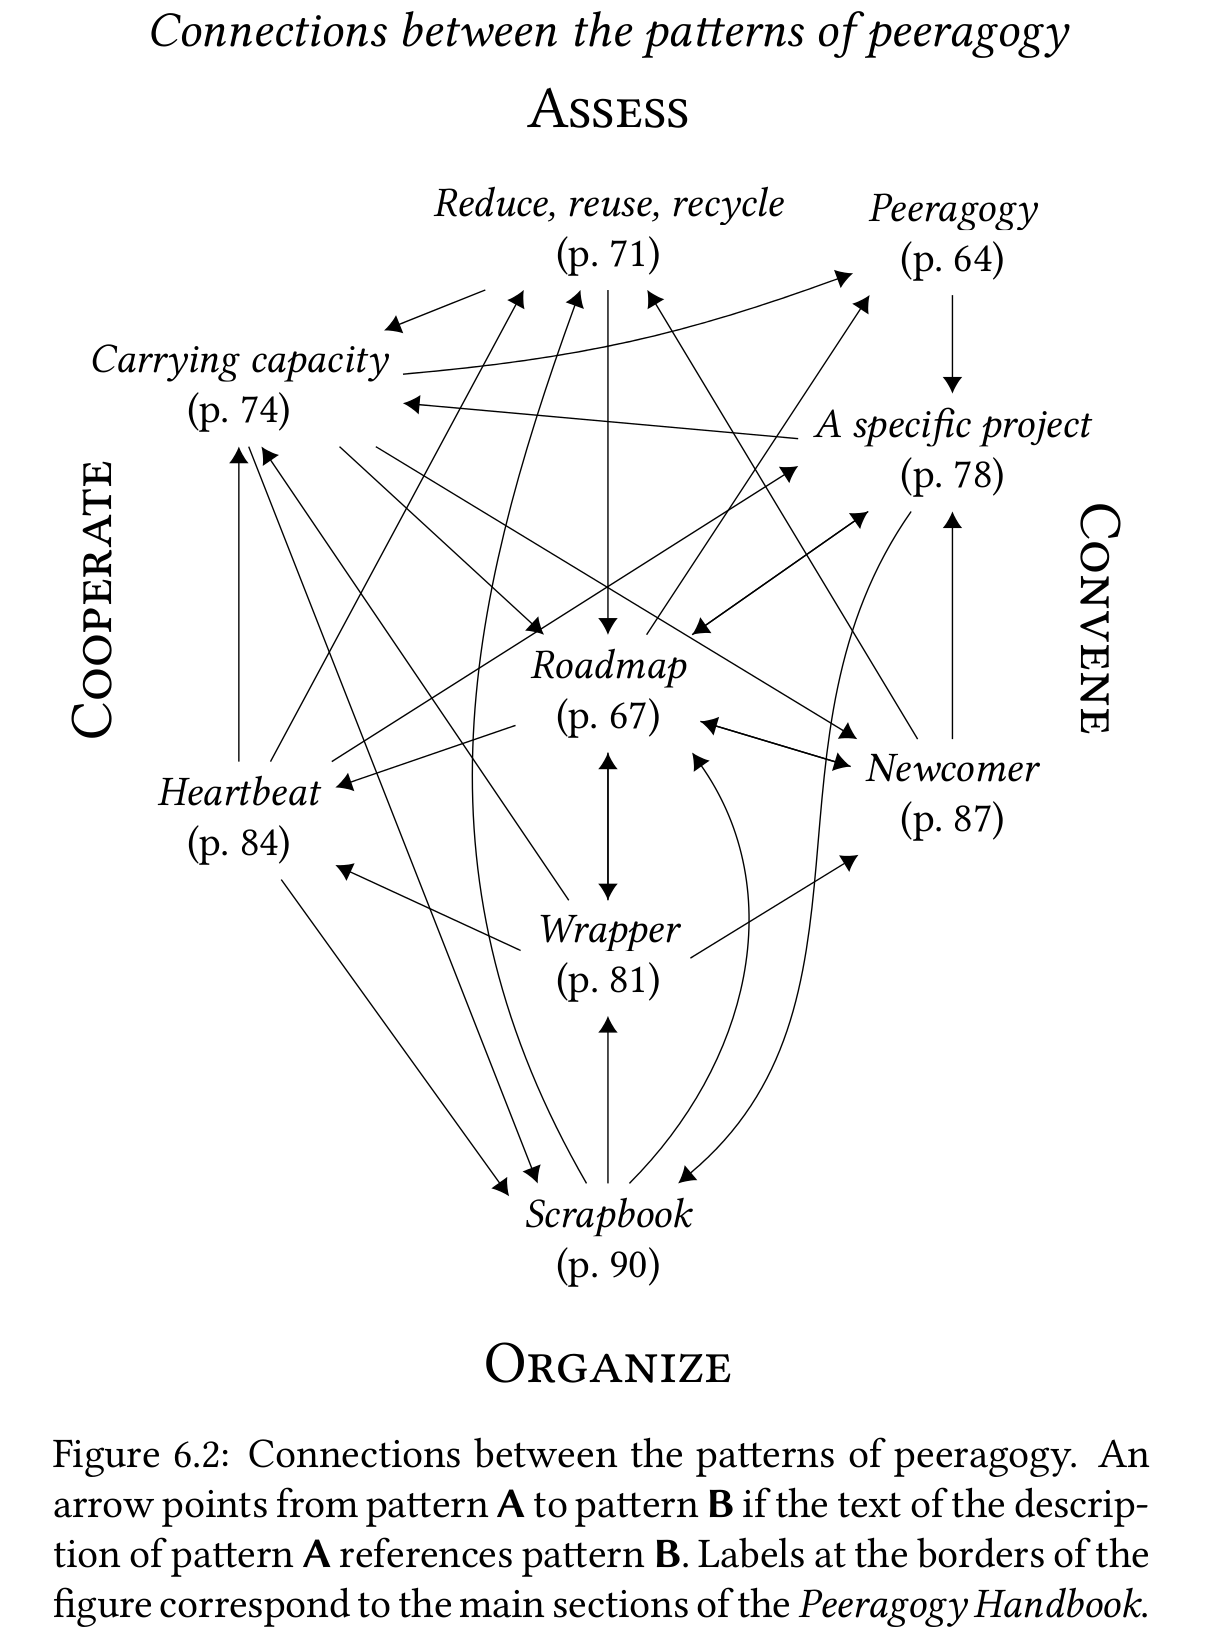
\includegraphics{images/pattern-connections.png}
\caption{image}
\end{figure}

\begin{longtable}[]{@{}l@{}}
\toprule
\begin{minipage}[b]{0.97\columnwidth}\raggedright
overview of problems and solutions in the pattern catalog\strut
\end{minipage}\tabularnewline
\midrule
\endhead
\begin{minipage}[t]{0.97\columnwidth}\raggedright
1. {{Peeragogy}}\strut
\end{minipage}\tabularnewline
\begin{minipage}[t]{0.97\columnwidth}\raggedright
\textbf{How can we find solutions together?} Get concrete about what the
real problems are.\strut
\end{minipage}\tabularnewline
\begin{minipage}[t]{0.97\columnwidth}\raggedright
2. {{Roadmap}}\strut
\end{minipage}\tabularnewline
\begin{minipage}[t]{0.97\columnwidth}\raggedright
\textbf{How can we get everyone on the same page?} Build a plan that we
keep updating as we go along.\strut
\end{minipage}\tabularnewline
\begin{minipage}[t]{0.97\columnwidth}\raggedright
3. {{Reduce, reuse, recycle}}\strut
\end{minipage}\tabularnewline
\begin{minipage}[t]{0.97\columnwidth}\raggedright
\textbf{How can we avoid undue isolation?} Use what's there and share
what we make.\strut
\end{minipage}\tabularnewline
\begin{minipage}[t]{0.97\columnwidth}\raggedright
4. {{Carrying capacity}}\strut
\end{minipage}\tabularnewline
\begin{minipage}[t]{0.97\columnwidth}\raggedright
\textbf{How can we avoid becoming overwhelmed?} Clearly express when
we're frustrated.\strut
\end{minipage}\tabularnewline
\begin{minipage}[t]{0.97\columnwidth}\raggedright
5. {{A specific project}}\strut
\end{minipage}\tabularnewline
\begin{minipage}[t]{0.97\columnwidth}\raggedright
\textbf{How can we avoid becoming perplexed?} Focus on concrete, doable
tasks.\strut
\end{minipage}\tabularnewline
\begin{minipage}[t]{0.97\columnwidth}\raggedright
6. {{Wrapper}}\strut
\end{minipage}\tabularnewline
\begin{minipage}[t]{0.97\columnwidth}\raggedright
\textbf{How can people stay in touch with the project?} Maintain a
summary of activities and any adjustments to the plan.\strut
\end{minipage}\tabularnewline
\begin{minipage}[t]{0.97\columnwidth}\raggedright
7. {{Heartbeat}}\strut
\end{minipage}\tabularnewline
\begin{minipage}[t]{0.97\columnwidth}\raggedright
\textbf{How can we make the project ``real'' for participants?} Keep up
a regular, sustaining rhythm.\strut
\end{minipage}\tabularnewline
\begin{minipage}[t]{0.97\columnwidth}\raggedright
8. {{Newcomer}}\strut
\end{minipage}\tabularnewline
\begin{minipage}[t]{0.97\columnwidth}\raggedright
\textbf{How can we make the project accessible to new people?} Let's
learn together with newcomers.\strut
\end{minipage}\tabularnewline
\begin{minipage}[t]{0.97\columnwidth}\raggedright
9. {{Scrapbook}}\strut
\end{minipage}\tabularnewline
\begin{minipage}[t]{0.97\columnwidth}\raggedright
\textbf{How can we maintain focus as time goes by?} Move things that are
not of immediate use out of focus.\strut
\end{minipage}\tabularnewline
\bottomrule
\end{longtable}

\hypertarget{references}{%
\subsection{References}\label{references}}

\begin{enumerate}
\def\labelenumi{\arabic{enumi}.}
\item
  Christopher Alexander, Sara Ishikawa, and Murray Silverstein. 1977.
  \emph{A Pattern Language: Towns, Buildings, Construction}. Oxford
  University Press, Oxford.
\item
  A.T. Ariyaratne. 1977. Organization of rural communities for group
  effort and self-help. \emph{Food Crisis Workshop, Los Banos, Laguna
  (Philippines), 7-9 Feb 1977}, 23--24. Retrieved from
  \url{http://www.sarvodaya.org/about/philosophy/collected-works-vol-1/rural-self-help}
\item
  Joseph Bergin, Jutta Eckstein, Markus Völter, et al.~2012.
  \emph{Pedagogical patterns: Advice for educators}. Joseph Bergin
  Software Tools, New York.
\item
  James O Coplien and B Woolf. 1997. A pattern language for writers'
  workshops. \emph{C++ report} 9: 51--60.
\item
  J. Corneli and A. Mikroyannidis. 2011. Crowdsourcing Education: A
  Role-Based Analysis. In \emph{Collaborative Learning 2.0: Open
  Educational Resources}, Alexandra Okada, Teresa Connolly and Peter
  Scott (eds.). IGI Global. Retrieved from
  \url{http://oro.open.ac.uk/33221/1/corneli_chap_okada_book.pdf}
\item
  J. Corneli, A. Jordanous, R. Shepperd, et al.~2015. Computational
  Poetry Workshop: Making Sense of Work in Progress. In
  \emph{Proceedings of the Sixth international conference on
  computational creativity, ICCC 2015}, Simon Colton, Hannu Toivonen,
  Michael Cook and Dan Ventura (eds.).
\item
  Joseph Corneli, Dorota Marciniak, Charles Jeffrey Danoff, et al.~2014.
  Building the Peeragogy Accelerator. \emph{Proceedings of OER14:
  Building communities of open practice}. Retrieved from
  \url{http://metameso.org/~joe/docs/Building_the_Peeragogy_Accelerator.pdf}
\item
  Merle Eugene Curti, Vernon Rosco Carstensen, Edmund David Cronon, and
  John William Jenkins. 1949. \emph{The University of Wisconsin, a
  history: 1848-1925}. Univ.~of Wisconsin Press.
\item
  Gilles Deleuze. {[}1968{]} 2004. \emph{Difference and repetition}.
  Bloomsbury Academic, London.
\item
  Neil B Harrison. 1999. The Language of Shepherding. \emph{Pattern
  Languages of Program Design} 5: 507--530.
\item
  Benjamin Mako Hill. 2013. Essays on Volunteer Mobilization in Peer
  Production. Retrieved from
  \url{http://dspace.mit.edu/handle/1721.1/86240}
\item
  Takashi Iba and Iba Laboratory. 2014. \emph{Learning Patterns: A
  Pattern Language for Creative Learning}. CreativeShift Lab, Yokohama.
\item
  Gerard Meszaros and Jim Doble. 1998. A pattern language for pattern
  writing. \emph{Pattern languages of program design} 3: 529--574.
\item
  Marvin Minsky. 1967. Why programming is a good medium for expressing
  poorly understood and sloppily formulated ideas. In \emph{Design and
  Planning II-Computers in Design and Communication}. 120--125.
\item
  PLAST Collective. 2015. The PLAST Project: Pattern Languages for
  Systemic Transformation. \emph{Spanda Journal} VI, 1: 205--218.
\item
  René Reiners, Ragnhild Halvorsrud, Aslak Wegner Eide, and Daniela
  Pohl. 2012. An approach to evolutionary design pattern engineering.
  \emph{Proceedings of the 19th Conference on Pattern Languages of
  Programs}.
\item
  Douglas Schuler. 2008. \emph{Liberating voices: A pattern language for
  communication revolution}. MIT Press, Cambridge, MA.
\item
  Till Schümmer, Joerg M Haake, and Wolfgang Stark. 2014. Beyond
  rational design patterns. \emph{Proceedings of the 19th european
  conference on pattern languages of programs}, ACM, 13 pp.
\item
  Booker T Washington. 1901. \emph{Up from slavery}. Doubleday \&
  Company, Inc.
\end{enumerate}

\begin{center}\rule{0.5\linewidth}{0.5pt}\end{center}
